% This is LLNCS.DEM the demonstration file of
% the LaTeX macro package from Springer-Verlag
% for Lecture Notes in Computer Science,
% version 2.4 for LaTeX2e as of 16. April 2010
%
\documentclass{llncs}
%
%\usepackage{ctex}
\usepackage{CJKutf8}
\usepackage{graphicx}
\usepackage{makeidx}  % allows for indexgeneration
\usepackage{amsmath}
\begin{document}
%
%\frontmatter          % for the preliminaries
%
%\pagestyle{headings}  % switches on printing of running heads

%\addtocmark{Hamiltonian Mechanics} % additional mark in the TOC

%
%\mainmatter              % start of the contributions
%
\title{A Relateness-Based Ranking Method for Knowledge-Based Question Answering}
%
\titlerunning{}  % abbreviated title (for running head)
%                                     also used for the TOC unless
%                                     \toctitle is used
%
\author{Han Ni\inst{1} \and Liansheng Lin\inst{2} \and Ge Xu\inst{3}}
%
%\authorrunning{Ivar Ekeland et al.} % abbreviated author list (for running head)
%
%%%% list of authors for the TOC (use if author list has to be modified)
%\tocauthor{Ivar Ekeland, Roger Temam, Jeffrey Dean, David Grove,
%Craig Chambers, Kim B. Bruce, and Elisa Bertino}
%
\institute{NetDragon Websoft Inc., Fuzhou, China \\
\email{nihan@nd.com.cn}
\and NetDragon Websoft Inc., Fuzhou, China \\
\email{linliansheng@nd.com.cn}
\and Minjiang University, Fuzhou, China \\
\email{xuge@pku.edu.cn}
}

\maketitle              % typeset the title of the contribution

\begin{abstract}
In this paper, we report technique details of our approach for the NLPCC 2018 
shared task knowledge-based question answering. Our system uses a word-based 
maximum matching method to find entity candidates. Then, we combine editor 
distance, character overlap and word2vec cosine similarity to rank SRO triples 
of each entity candidate. Finally, the object of the top 1 score SRO is 
selected as the answer of the question . The result of our system achieves 
62.94\% of answer exact matching on the test set.

\keywords{Question answer, Knowledge base, Entity linking, Relation Ranking}
\end{abstract}

\section{Introduction}
Automatic open-domain quesion answering has attracted great attention with the 
development of Natural Language Processing (NLP) and Information Retrieval (IR) 
techniques. One of the typical tasks named Knowledge-Based Quetion Answering 
(KBQA) is defined to retrieve a specific entity from knowledge base as the 
answer to a given question. 

The challenge of retrieval-based KBQA is how to match unstructured natural
language questions with structured data in knowledge base. To understand a 
question, it is necessary to figure out the topic entity and relation chain 
inside the question. Thus, topic entity linking and relation ranking are the 
most important modules in our system.

\section{Related Work}
% \cite{Author}
Knowledge-based question answering is a challenging task in the field of NLP. 
The mainstream approaches can be divided into three categories: semantic 
parsing based\cite{Zettlemoyer}\cite{Kwiatkowski}\cite{Liang}\cite{Berant1}
\cite{Berant2}, information extraction based \cite{Bast}\cite{Fader}
\cite{Yao} and retrieval based \cite{Bordes}\cite{Bordes2}\cite{Dong}.

The semantic parsing based approaches translate natural language questions into a
series of semantic representations in logic forms. They query the answer in knowledge
base through the corresponding query statement. Yih et al.\cite{Yih} present a semantic
parsing method via staged query graph generation. Convolution neural network is used
to calculate the similarities between question and relation chains.

The information extraction based approaches extract topic entities from questions
and generate a knowledge base subgraph with the topic entity node as the center. Each
node in the subgraph can be used as a candidate answer. By examining the questions
and extracted information according to some rules or templates, they obtain the feature
vectors of the questions. A classifier is then constructed to filter candidate answers
based on input feature vectors. Yao and Van Durme \cite{Yao2} associate question features
with answer patterns described by Freebase. They also exploit ClueWeb, mined
mappings between knowledge base relations and natural language text, and show that it
helps both relation prediction and answer extraction.

The idea of retrieval-based method is similar to that of information extraction based
methods. The question and candidate answers are mapped to distributed representation.
The distributed representations are trained on labeled data, aiming to optimize the
matching function between the question and the correct answer. Zhang et al. \cite{Zhang}
combine bi-directional LSTM with an attention mechanism to represent the questions
dynamically according to diverse focuses of various candidate answers.

These approaches work well on the English open dataset WebQuestion. However,
their performances on a Chinese KBQA dataset have not been presented before.

\section{Our Approach}
% nlpcc2018-kbqa-workflow.png
Figure 1 shows the system architecture of our approach. For each question, the 
system finds the entity candidates firstly. And then entity ranking and relation 
ranking are conducted seperately to assign each entity candidate and relation a
rank score. Finally, in the answer ranking stage, the system finds the top 1 
triple according to the entity score and relation score. The object entity 
of the top 1 triple is the answer of the quesiton.
\begin{figure}
\centering
  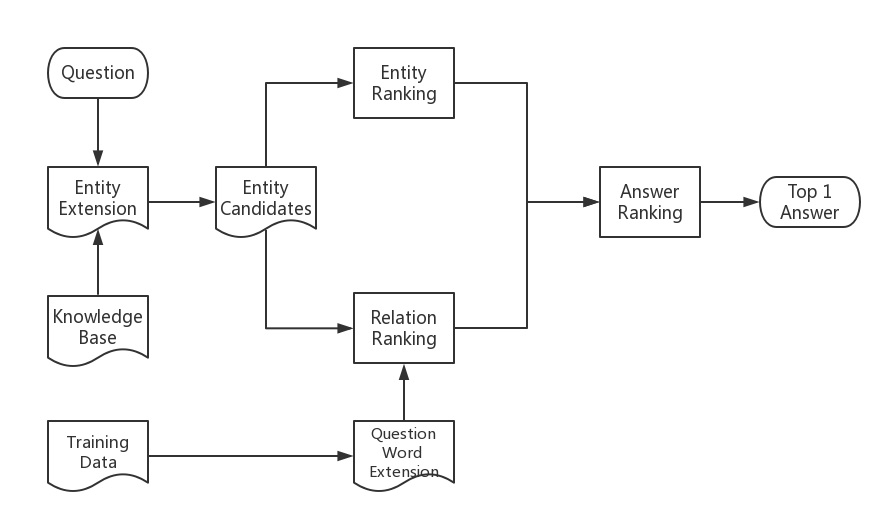
\includegraphics[width=4in]{nlpcc2018-kbqa-workflow.png}
  \caption[width=\textwidth]{System architecture}
\end{figure}

\subsection{Entity Linking}

Since the entity in the knowledge base has various name, such as Chinese name, 
English name, nick name, alias and so on, we build a Entity Map which mapps 
these names to the original entity.

In order to detect the topic entity in the question, we use a word-based maximum 
matching method to find entity candidates. First of all, the question is 
segmented by ltp\footnotemark\ \cite{Wanxiang} segmenter. Then, we join the words in the 
question one by one and search it in the Entity Map. If it exists in the 
keys of Entity Map, the corresponding value to the key will be added to a 
entity candidates list.
\footnotetext{http://ltp.ai/}

Here is an example:

Consider the question, \begin{CJK}{UTF8}{gbsn}
马丁·泰勒青少年时在哪支球队踢球
\end{CJK}.
After segmentation, we get a list of words \begin{CJK}{UTF8}{gbsn}
马丁·泰勒, 青少年, 时, 在, 哪, 支, 球队, 踢球
\end{CJK}. Then we filter stop words \begin{CJK}{UTF8}{gbsn}
时, 在, 支
\end{CJK} and question words \begin{CJK}{UTF8}{gbsn}
哪
\end{CJK}, because they are impossible to be part of entity. After that, 
two sub-list of words are left, which are \begin{CJK}{UTF8}{gbsn}
马丁·泰勒, 青少年
\end{CJK} and \begin{CJK}{UTF8}{gbsn}
球队, 踢球
\end{CJK}. Then, we do word-based maximum matching for each sub-list. 
For sub-list, \begin{CJK}{UTF8}{gbsn}
马丁·泰勒, 青少年
\end{CJK}, we first join all the words (\begin{CJK}{UTF8}{gbsn}
马丁·泰勒青少年
\end{CJK}) and search it in the Entity Map. Apparently, it is not a entity. 
Then, we shorten the string length by one. Now, we search \begin{CJK}{UTF8}{gbsn}
马丁·泰勒
\end{CJK} and \begin{CJK}{UTF8}{gbsn}
青少年
\end{CJK} in the Entity Map separately. They are both existing entity, so they 
are added to the entity candidates list. For sub-list \begin{CJK}{UTF8}{gbsn}
球队, 踢球
\end{CJK}, we conduct the same operation. In the end, we get entity candidates: \\
\begin{CJK}{UTF8}{gbsn}
马丁·泰勒 \\ 
马丁·泰勒(英国足球运动员) \\ 
马丁·泰勒(英国足球评论员) \\
青少年 \\
《青少年》(2007年英国电影) \\ 
青少年(按年龄划分的社会群体) \\
青少年(2011年贾森·雷特曼导演美国电影) \\
踢球
\end{CJK}


\subsection{Ranking}

The knowledge base consists of millions of Subject-Relation-Object (SRO) 
triples. Each subject entity has dozens of Relation-Object pairs, each relation 
corresponding to only one object entity. Therefore, finding the answer to the 
question is equal to rank the relations of the subject entity and the object 
entity corresponding to the top one relation is supposed to be the answer.

After entity candidates have been found in the entity linking section, we can 
now collect all SRO triples of theses entities from the knowledge base. In this 
section, we combine editor distance score, character overlap score and word2vec 
cosine similarity score to rank each entity candidate and their relations.

\subsubsection{Edit Distance}
The edit distance is a way of quantifying how dissimilar two strings are to one 
another by counting the minimum number of operations required to transform one 
string into the other. The edit distance score we used is a variant of the 
original edit distance. Suppose that the original edit distance of two strings 
$s_1$ and $s_2$ is notated as $ ed(s_1, s_2) $, the edit distance score we use is

  \begin{equation}
    score_{ed} = 1 - \frac{ed(s_1, s_2)}{max(len(s_1), len(s_2))}
  \end{equation}

\subsubsection{Character Overlap}
The character overlap is the number of overlapped characters in two strings. 
Greater character overlap suggests that the two strings are more topic related.
We notate the character overlap score as $ score_{co} $.

\begin{equation}
    score_{co} = \frac{|set(s_1)| \cap |set(s_2)|}{|set(s_1)| \cup |set(s_2)|}
  \end{equation}

\subsubsection{Word2vec Cosine similarity}
We train a word2vec model with a 20G chinese news corpus so that we can obtain a 
vector for each chinese word in the vocabulary. Then the string vector is 
computed as
\begin{equation}
    v(s) = \sum_{w_i \in s}{v(w_i)}
  \end{equation}
so the word2vec cosine similarity of two strings is computed as the cosine 
similarity of two string vectors.
\begin{equation}
    score_{w2v} = \frac{v(s_1) \cdot v(s_2)}{||v(s_1)|| \cdot ||v(s_2)||}
  \end{equation}

\subsubsection{Related score}
The related score of two string is defined as:
\begin{equation}
    score_{related} = score_{ed} + score_{co} + score_{w2v}
  \end{equation}

\subsubsection{Entity Ranking}
We rank entity candidate by how many object entity of the candidate are related 
with question.

Consider the question \begin{CJK}{UTF8}{gbsn}
巴西球员托罗是哪天出生的
\end{CJK}. Suppose that there are more than one entities \begin{CJK}{UTF8}{gbsn}
托罗
\end{CJK} in the knowledge base and they have different nationalities such as 
\begin{CJK}{UTF8}{gbsn}
波多黎各, 墨西哥, 巴西
\end{CJK} etc. and different occupations such as \begin{CJK}{UTF8}{gbsn}
球员, 导演, 演员
\end{CJK} etc. When we calculate the related score of each entity candidate and 
the question, apparently the related score of the entity of which the nationality
is \begin{CJK}{UTF8}{gbsn}
巴西
\end{CJK} and the occupation is \begin{CJK}{UTF8}{gbsn}
球员
\end{CJK} will be higher than that of others. In experience, 
if the related score is greater than a threshold $\lambda$, then we think that the object entity 
is related with the question. So entity score is computed as
\begin{equation}
    score_{award} = (1+score_{ed}) \times (1+score_{co}) \times (1+score_{w2v})
  \end{equation}
\begin{equation}
    score_{S} =  1 \times \prod_{o \in S}{score_{award}(O, Q)}
  \end{equation}
\begin{equation}
    score_{award}(O, Q) = \begin{cases} 
                          score_{award}(O, Q) & score_{award}(O, Q) \geq \lambda \\
                          1 & score_{award}(O, Q) < \lambda \\
                          \end{cases}
  \end{equation}
We tune the value of $\lambda$ from 1.0 to 2.0, gap 0.1, and find that when 
$\lambda = 1.5$ it achieves the best result on the training data.


\subsubsection{Relation Ranking}

Before calculating the score, we remove the string corresponding to the entity 
candidate and related object entity for simplifying the computation. For 
example, after removing the string, the question \begin{CJK}{UTF8}{gbsn}
巴西球员托罗是哪天出生的
\end{CJK} becomes \begin{CJK}{UTF8}{gbsn}
是哪天出生的
\end{CJK}.

In addition, we also do question word extension. In some cases, the relation of 
entity does not appear in the question. For example, the relation to the question
is supposed to be \begin{CJK}{UTF8}{gbsn}
出生日期
\end{CJK} or \begin{CJK}{UTF8}{gbsn}
生日
\end{CJK} (both refers to "birthday" in English), however, neither of them 
exists in the question. So, we map \begin{CJK}{UTF8}{gbsn}
哪天出生
\end{CJK} to \begin{CJK}{UTF8}{gbsn}
出生日期
\end{CJK} and \begin{CJK}{UTF8}{gbsn}
生日
\end{CJK}, the latter is called the extension of question word. 

Finally, we rank relations of each entity candidate by caculating the related 
score of each relation with the quesiton and the extension of question word.
\begin{equation}
    score_{R} = \alpha * score_{related}(R, Ext) + 
                       \beta * score_{related}(R, Q \cup Ext)
  \end{equation}
where, $R$ refers to relation, $Ext$ refers to 
the extension of question word, and $Q \cup Ext$ refers to the union of question and $ext$. The $\alpha$ and $\beta$ are weight factors. We 
set $\alpha$ to be 0.47 and $\beta$ to be 0.53 according to the experiment.

\subsubsection{Answer Ranking}
For a SRO triple, we caculate the score as below:
\begin{equation}
    score_{SRO} = score_{R} \times score_{S}
  \end{equation}
\begin{equation}
    score_{S} = \begin{cases} 
                          score_{S} & score_{award}(O, Q) < \lambda \\
                          1 & score_{award}(O, Q) \geq \lambda \\
                          \end{cases}
  \end{equation}
where O refers to Object of SRO triple, Q refers to the question and $\lambda$ 
is set to be 1.5 according to the experiment. 

If the $score_{award}(O, Q) \geq \lambda$, it suggests that 
the object is a known fact and can not be the answer of the question shown as Eq(11). 

We rank SRO by multiplying the score of each relation and the score 
of corresponding entity candidate and get the Object from the top 1 SRO as the answer.



\section{Experiments}

\subsection{Dataset}

In this paper, we use the dataset provided by the NLPCC 2018 open domain KBQA
shared task. The dataset includes 24,479 single-relation question-answer pairs for
training, a Chinese knowledge base with 43M SRO triples, and 7M mapping data from
mentions to entities. The test set contains 618 questions. 

Since the mapping data is not what our system desires, we rebuild a Entity Map 
from mentions to entities with no word segmentation.

\subsection{Setup}
The word embeddings used in our system is pre-trained by gensim\footnotemark\ . We use the 
skip-gram model \cite{Mikolov} and the dimension is set to be 300.
\footnotetext{https://radimrehurek.com/gensim/}

\subsection{Results}
The results of our system achieves 62.94\% of answer exact matching on the test 
set, which ranks 3rd place in the final leaderboard.

\subsection{Error Analysis}
We analyze the causes of the error cases (229 in total). 37.6\% of errors are 
caused by entity linking and 27.9\% are caused by relation ranking. 16.6\% of 
errors are attributed to that the desire answer of the quesiton is the subject 
entity of the SRO triple and we can not use object entity to infer subject entity. 

In addition, 5.2\% of errors are caused by the confliction of knowledge base. 
For example, to the question \begin{CJK}{UTF8}{gbsn}国脚黄博文在场上司职什么角色?\end{CJK}, our answer is \begin{CJK}{UTF8}{gbsn} 
中场\end{CJK}, while the official answer is \begin{CJK}{UTF8}{gbsn} 
前卫\end{CJK}. However, in the knowledge base, the entity \begin{CJK}{UTF8}{gbsn} 
黄博文\end{CJK} contains both triples \begin{CJK}{UTF8}{gbsn} 
黄博文\end{CJK} $|||$ \begin{CJK}{UTF8}{gbsn}场上位置\end{CJK} $|||$ \begin{CJK}{UTF8}{gbsn}中场\end{CJK} and \begin{CJK}{UTF8}{gbsn} 
黄博文\end{CJK} $|||$ \begin{CJK}{UTF8}{gbsn}位置\end{CJK} $|||$ \begin{CJK}{UTF8}{gbsn}前卫\end{CJK}. 

For the last 16.6\% of errors, in fact, we 
find the correct answers, but the offical system judge them as incorrect ones. 
For example, to the question \begin{CJK}{UTF8}{gbsn}泰国武里南联队是哪年成立的?\end{CJK}, 
our answer is \begin{CJK}{UTF8}{gbsn} 
1970年\end{CJK}, while the official answer is \begin{CJK}{UTF8}{gbsn} 
1970\end{CJK}. And in the preprocessing stage, we convert all characters in the 
knowledge base from full-width to half-width and convert all upper case letter 
to lower case, which also cause the official 
system to judge our correct answer as wrong one. For example, to the question \begin{CJK}{UTF8}{gbsn}牛津联足球俱乐部的主席是谁?\end{CJK}, 
our answer is \begin{CJK}{UTF8}{gbsn} 
达利尔·伊尔斯 (darryl eales)\end{CJK}, while the official answer is \begin{CJK}{UTF8}{gbsn} 
达利尔·伊尔斯 (Darryl Eales)\end{CJK}. If these cases caused by wrong judgement and 
knowledge base confliction are revised, the answer exact matching of our results 
will be 69.42\%.

\section{Conclusion}

In this paper, we report technique details of our approach for the NLPCC 2018 
shared task knowledge-based question answering. Our system uses a word-based 
maximum matching method to find entity candidates. Then, we combine editor 
distance, character overlap and word2vec cosine similarity to rank SRO triples 
of each entity candidate and get the object of the top 1 score SRO as the 
answer of the question. 

We also try to use deep learning in entity linking 
and question-relation match. However, for entity linking, since the questions 
of test set are greatly different from that of training set, the model can not 
generalize from training data to test data. For question-relation match 
problem, it seems to be quite difficult to match thousands of questions to 
millions of relations, even by deep learning. And the number of relations in 
the training set is 4,385, however the number of that in the knowldge base is 
up to 587,576. It is impractical to train a relation match model from such a 
small dataset. Even though, after replacing the provided mention2id with the 
entity extension built by us and revising some errors in the knowledge base, we 
also achieve good results with statistic and rule-based methods.

%
% ---- Bibliography ----
%
\begin{thebibliography}{5}

\bibitem {Zettlemoyer}
Zettlemoyer, L.S., Collins, M.: Learning to map sentences to logical form: structured
classification with probabilistic categorial grammars. In: UAI (2005)

\bibitem {Kwiatkowski}
Kwiatkowski, T., Zettlemoyer, L., Goldwater, S., Steedman, M.: Inducing probabilistic CCG
grammars from logical form with higher-order unification. In: EMNLP (2010)

\bibitem {Liang}
Liang, P., Jordan, M.I., Klein, D.: Learning dependency-based compositional semantics. In:
ACL (2011)

\bibitem {Berant1}
Berant, J., Chou, A., Frostig, R., Liang, P.: Semantic parsing on freebase from
question-answer pairs. In: EMNLP (2013)

\bibitem {Berant2}
Berant, J., Liang, P.: Semantic parsing via paraphrasing. In: ACL (2014)

\bibitem {Bast}
Bast, H., Haussmann E.: More accurate question answering on freebase. In: Information and
Knowledge Management (2015)

\bibitem {Fader}
Fader, A., Zettlemoyer, L., Etzioni, O.: Open question answering over curated and extracted
knowledge bases. In: Knowledge Discovery and Data Mining (2014)

\bibitem {Yao}
Yao, X.: Lean question answering over freebase from scratch. In: ACL (2015)

\bibitem {Bordes}
Bordes, A., Chopra, S., Weston, J.: Question answering with subgraph embeddings. In:
EMNLP (2014)

\bibitem {Bordes2}
Bordes, A., Weston, J., Usunier, N.: Open question answering with weakly supervised
embedding models. In: ECML (2014)

\bibitem {Dong}
Dong, L., Wei, F., Zhou, M., Xu, K.: Question answering over freebase with multi-column
convolutional neural networks. In: ACL (2015)

\bibitem {Yih}
Yih, W., Chang, M.-W., He, X., Gao, J.: Semantic parsing via staged query graph
generation: question answering with knowledge base. In: ACL (2015)

\bibitem {Yao2}
Yao, X., Van Durme, B.: Information extraction over structured data: question answering
with freebase. In: ACL (2014)

\bibitem {Zhang}
Zhang, Y., Liu, K., He, S., Ji, G., Liu, Z., Wu, H., Zhao, J.: Question answering over
knowledge base with neural attention combining global knowledge information. arXiv:1606.
00979 (2016)

\bibitem {Wanxiang}
Wanxiang Che, Zhenghua Li, Ting Liu. LTP: A Chinese Language Technology Platform. In Proceedings of the Coling 2010:Demonstrations. 2010.08, pp13-16, Beijing, China. 

\bibitem {Mikolov}
Mikolov, T., Chen, K., Corrado, G., Dean, J.: Efficient estimation of word representations in
vector space. Comput. Sci. (2013)
\end{thebibliography}

\end{document}



